%%%%%%%%%%%%%%%%%%%%%%%%%%%%%%%%%%%%%%%%%
% Beamer Presentation
% LaTeX Template
% Version 1.0 (10/11/12)
%
% This template has been downloaded from:
% http://www.LaTeXTemplates.com
%
% License:
% CC BY-NC-SA 3.0 (http://creativecommons.org/licenses/by-nc-sa/3.0/)
%
%%%%%%%%%%%%%%%%%%%%%%%%%%%%%%%%%%%%%%%%%

%----------------------------------------------------------------------------------------
%	PACKAGES AND THEMES
%----------------------------------------------------------------------------------------

\documentclass{beamer}

\mode<presentation> {

% The Beamer class comes with a number of default slide themes
% which change the colors and layouts of slides. Below this is a list
% of all the themes, uncomment each in turn to see what they look like.

%\usetheme{default}
%\usetheme{AnnArbor}
%\usetheme{Antibes}
%\usetheme{Bergen}
%\usetheme{Berkeley}
%\usetheme{Berlin}
%\usetheme{Boadilla}
%\usetheme{CambridgeUS}
%\usetheme{Copenhagen}
%\usetheme{Darmstadt}
%\usetheme{Dresden}
%\usetheme{Frankfurt}
%\usetheme{Goettingen}
%\usetheme{Hannover}
%\usetheme{Ilmenau}
%\usetheme{JuanLesPins}
%\usetheme{Luebeck}
%\usetheme{Madrid}
%\usetheme{Malmoe}
%\usetheme{Marburg}
%\usetheme{Montpellier}
%\usetheme{PaloAlto}
%\usetheme{Pittsburgh}
%\usetheme{Rochester}
%\usetheme{Singapore}
%\usetheme{Szeged}
\usetheme{Warsaw}

% As well as themes, the Beamer class has a number of color themes
% for any slide theme. Uncomment each of these in turn to see how it
% changes the colors of your current slide theme.

%\usecolortheme{albatross}
%\usecolortheme{beaver}
%\usecolortheme{beetle}
%\usecolortheme{crane}
%\usecolortheme{dolphin}
%\usecolortheme{dove}
%\usecolortheme{fly}
%\usecolortheme{lily}
%\usecolortheme{orchid}
\usecolortheme{rose}
%\usecolortheme{seagull}
%\usecolortheme{seahorse}
%\usecolortheme{whale}
%\usecolortheme{wolverine}

%\setbeamertemplate{footline} % To remove the footer line in all slides uncomment this line
%\setbeamertemplate{footline}[page number] % To replace the footer line in all slides with a simple slide count uncomment this line

%\setbeamertemplate{navigation symbols}{} % To remove the navigation symbols from the bottom of all slides uncomment this line
}

\usepackage{graphicx} % Allows including images
\usepackage{booktabs} % Allows the use of \toprule, \midrule and \bottomrule in tables
\usepackage{polski}
\usepackage[utf8]{inputenc}
\usepackage{xmpmulti}
\usepackage{animate}
\usepackage{array}



%----------------------------------------------------------------------------------------
%	TITLE PAGE
%----------------------------------------------------------------------------------------

\title{Pytania -- egzamin inżynierski} % The short title appears at the bottom of every slide, the full title is only on the title page

\author{Lidia J. Opuchlik} % Your name
\institute[PJATK] % Your institution as it will appear on the bottom of every slide, may be shorthand to save space
{
Polsko -- Japońska Akademia Technk Komputerowych \\ % Your institution for the title page
\medskip
\textit{s16478@pjwstk.edu.pl} % Your email address
}
\date{\today} % Date, can be changed to a custom date



\newenvironment<>{varblock}[2][1\textwidth]{%
	\setlength{\textwidth}{#1}
	\begin{actionenv}#3%
			\def\insertblocktitle{#2}%
			\par%
			\usebeamertemplate{block begin}}
		{\par%
			\usebeamertemplate{block end}%
	\end{actionenv}
}

\begin{document}


\begin{frame}
\titlepage % Print the title page as the first slide
\end{frame}

\begin{frame}
\frametitle{Agenda} % Table of contents slide, comment this block out to remove it
\tableofcontents % Throughout your presentation, if you choose to use \section{} and \subsection{} commands, these will automatically be printed on this slide as an overview of your presentation
\end{frame}

%----------------------------------------------------------------------------------------
%	PRESENTATION SLIDES
%----------------------------------------------------------------------------------------

%-------------------------------  SEKCJA O TWIERDZENIU BAYESA   -----------------
\section{Pytanie nr 8} % Sections can be created in order to organize your presentation into discrete blocks, all sections and subsections are automatically printed in the table of contents as an overview of the talk
%------------------------------------------------

\subsection{Twierdzenie Bayesa.} % A subsection can be created just before a set of slides with a common theme to further break down your presentation into chunks

\begin{frame}
	\frametitle{Twierdzenie Bayesa}
	\begin{center}
		{\Huge Twierdzenie Bayesa}
	\end{center}
\end{frame}


\begin{frame}
	\frametitle{Twierdzenie Bayesa}
	\begin{enumerate}
		\item Thomas Bayes, presbiteriański pastor, statystyk, filozof w 18-wiecznej Anglii.
		\item Mówi o \textbf{prawdopodobieństwie warunkowym}. Pozwala określić prawdopodobieństwo zajścia jakiegoś zdarzenia, o ile zaszło jakieś inne zdarzenie. \\ 
	\end{enumerate}
	
	\begin{block}{Treść (dla dwóch zdarzeń)}
		
			\begin{equation*}
					P (A|B) = \dfrac{P (B|A) \cdot P (A)}{P (B)}, \qquad oraz \  P(B) > 0 \ i \ P(A) \geq 0
			\end{equation*}
		

		{\scriptsize gdzie: } \\
		{\tiny
			$P (A|B)$ -- prawdopodobieństwo zajścia zdarzenia A, gdy zachodzi zdarzenie B (posterior probability), \\
			$P (B|A)$ -- prawdopodobieństwo zajścia zdarzenia B, gdy zachodzi zdarzenie A (likelihood), \\
			$P (A)$ -- prawdopodobieństwo zajścia zdarzenia A (prior probability), \\
			$P (B)$ -- prawdopodobieństwo zajścia zdarzenia B (evidence). \\
		}
	\end{block}
	

\end{frame}


%% ---- DOWÓd

\begin{frame}
	\frametitle{Dowód (dla dwóch zdarzeń*)}
		\begin{figure}
			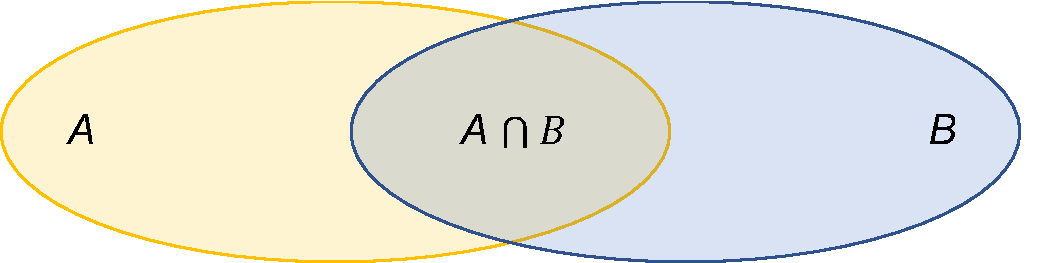
\includegraphics[width=0.7\textwidth]{bayes}
				\caption{{\tiny Iloczyn zbiorów A i B.}}
		\end{figure}
	Z definicji: \\	
	\begin{center}
		$P (A|B) = \dfrac{P (A \cap B)}{P (B)}  \Leftrightarrow P (A \cap B) = P (A|B) \cdot P (B)$\\
		\bigskip
		$P (B|A) = \dfrac{P (A \cap B)}{P (A)} \Leftrightarrow P (A \cap B) = P (B|A) \cdot P (A)$ \\
		\end{center}
\end{frame}

\begin{frame}
	\frametitle{Dowód c. d.}
		\begin{center}
				$P (A \cap B) = P (A|B) \cdot P (B)$\\
				\bigskip
				$P (A \cap B) = P (B|A) \cdot P (A)$ \\
				\bigskip
				$P (A|B) \cdot P (B) = P (B|A) \cdot P (A)$ \\
				\bigskip
				$\Downarrow$ \\
				\bigskip
				$\boxed{P (A|B) = \dfrac{P (B|A) \cdot P (A)}{P (B)}}$
		\end{center}
{\tiny \bigskip *dowód dla wiekszej liczby zdarzeń jest dużo bardziej skomplikowany}
\end{frame}

%% ---- PRZYKLAD

\begin{frame}
	\frametitle{Trywialny przykład}
	\textbf{Treść zadania: }\\
	Obliczyć prawdopodobieństwo, że osoba jest chora na grypę, gdy występuje u niej gorączka, wiedząc, że: zdarzenie A -- osoba jest chora na grypę, zdarzenie B -- u osoby występuje gorączka. W zadaniu dane są następujące prawdopodobieństwa: $P(B|A)$~=~0.7, $P(A)$ = 0.1, $P(B)$ = 0.2. \\
	\bigskip
	\textbf{Rozwiązanie: }\\
	Korzystając ze wzoru Bayesa obliczamy $P(grypa|goraczka)$: \\
	\bigskip
\begin{center}
		$P (grypa|goraczka) = \dfrac{P (goraczka|grypa) \cdot P (grypa)}{P (goraczka)} $  \\
	\bigskip
		$P (grypa|goraczka) = \dfrac{0.7 \cdot 0.1}{0.2} = \textbf{0.35}$ \\
\end{center}
\end{frame}


\begin{frame}
	\frametitle{Nieco bardziej złożony przykład}
{\footnotesize Klasyczny przykład zastosowania twierdzenia Bayesa, to przypadek testowania na dosyć rzadką chorobę. Szukamy jakie jest prawdopodobieństwo, że osoba jest chora, jeżeli wyszedł jej pozytywny wynik testu. Precyzja testu to 95~\%. \\
Intuicyjnie nasuwa się, że prawdopodobieństwo wynosi 0.95. Jest to jednak błędne myślenie. \\
\bigskip
{\small \textbf{Analiza: \\}}

\begin{center}
		$P (choroba|pozytywny) = \dfrac{P (pozytywny|choroba) \cdot P (choroba)}{P (pozytywny)} $  \\
\end{center}
\bigskip
}
{\scriptsize \textbf{P(choroba$|$pozytywny)} -- prawdopodobieństwo, że osoba ma chorobę bazując na tym, że test wyszedł pozytywny. \\

\textbf{P(pozytywny$|$choroba)} -- prawdopodobieństwo, że test wyszedł pozytywnie jeżeli rzeczywiście jest zdiagnozowana choroba. Mówi ono o czułości testu — true positive (95~\%) oraz specyficzności testu — true negative (95~\%). \\

\textbf{P(choroba)} -- prawdopodobieństwo wystąpienia choroby u danej osoby. Załóżmy, że choruje 1/100 osób; P = 0.01. \\

\textbf{P(pozytywny)} -- prawdopodobieństwo, że testowana osoba będzie miała wynik pozytywny. Może być tak, że test da prawidłowy wynik (true positive) lub zakłamany wynik (false positive). \\}
\end{frame}
\begin{frame}
	\begin{center}
		$P (choroba|pozytywny) = \dfrac{0.95 \cdot 0.01}{(0.01\cdot 0.95) + (0.99 \cdot 0.05)} = $
		\bigskip
		$= \dfrac{0.0095}{0.0095 + 0.0495} = \dfrac{0.0095}{0.059} = 0.1610169… = 16~\%$  \\
	\end{center}
Jaki to ma sens? Jedynie 16~\% osób z wynikiem pozytywnym ma chorobę.\\
\end{frame}

\begin{frame}
	\frametitle{W czym  przydatne jest twierdzenie Bayesa?}
	\begin{enumerate}
		\item stosowane do lepszego zrozumienia danych
		\item ułatwia zrozumienie i interpretację wyników testów A/B
		\item w machine learningu -- algorytmy -- Naive Bayes, Optymalny Klasyfikator Bayesowski, optymalizacja Bayesowska, Bayesowskie sieci przekonań (Bayesian Belief Networks)
		
	\end{enumerate}
	
\end{frame}




%--------------  SEKCJA O WYSZUKIWANIU I SORTOWANIU   -----------------


\section{Pytanie nr 22} % Sections can be created in order to organize your presentation into discrete blocks, all sections and subsections are automatically printed in the table of contents as an overview of the talk
%------------------------------------------------

\subsection{Najważniejsze algorytmy wyszukiwania i sortowania.} 
% Przegląd i zastosowania
% A subsection can be created just before a set of slides with a common theme to further break down your presentation into chunks
\subsubsection{Wyszukiwanie} 
\subsubsection{Sortowanie} 

\begin{frame}
	\frametitle{Wyszukiwanie i sortowanie}
\begin{center}
		{\Huge Najważniejsze algorytmy wyszukiwania i sortowania}
\end{center}
\end{frame}


\begin{frame}
	\frametitle{Wyszukiwanie i sortowanie}
	
	\begin{minipage}{0.35\textwidth}
		\textbf{Wyszukiwanie}
		\begin{enumerate}
			\item liniowe
			\item binarne
			\item skok co k-ty element
		\end{enumerate}
	\end{minipage}
	\hspace{0.1cm}
	\begin{minipage}{0.55\textwidth}
		\textbf{Sortowanie}
		\begin{enumerate}
			\item przez wybieranie (selection sort)
			\item bąbelkowe (bubble sort)
			\item przez scalanie (merge sort)
			\item szybkie (quick sort)
			\item przez wstawianie (insertion sort)
			\item zliczeniowe (counting sort)
		\end{enumerate}
	\end{minipage}
\end{frame}


\begin{frame}
	\frametitle{Wyszukiwanie}
		\begin{center}
				{\Huge Wyszukiwanie}
		\end{center}
\end{frame}


\begin{frame}
	\frametitle{Wyszukiwanie -- na czym polega?}

		Polega na odszukaniu elementu o danej wartości (klucza) w nieposortowanej lub posortowanej strukturze danych (tablicy lub liście) i zwrócenie indeksu, pod którym znaleziony element się znajduje*. Jeżeli element nie zostanie znaleziony, wyświetlany jest stosowny komunikat (często wartość -1). \\
		\bigskip
		{\tiny *Jeżeli jest kilka takich samych elementów w ciągu, to zwracany jest indeks pierwszego napotkanego. \\
		** klucz i indeksy są liczbami całkowitymi\\
		}
\end{frame}

\begin{frame}
	\frametitle{Wyszukiwanie liniowe}
	\begin{block}{Na czym polega??}
	1. Wartości kolejnych elementów ciągu zaczynając od tego pod indeksem 0 a kończąc na n-1 porównuje się z wartością klucza.\\
	2. Zwraca się indeks znalezionego elementu, bądź -1 w przypadku gdy nie został on znaleziony.
\end{block}
	\begin{itemize}
	\item struktura danych \textbf{nie musi} być posortowana
	\item pesymistyczna złożoność O(n)
\end{itemize}
\end{frame}

\begin{frame}
	\frametitle{Wyszukiwanie binarne}
		\begin{block}{Na czym polega??}
		1. W posortowanym ciągu porównuje się wartość klucza z wartością środkowego elementu. Jeżeli są takie same, zwracany jest indeks. \\
		2a. Jeżeli klucz $<$ środkowy element, to ogranicza się dalsze przeszukiwanie do lewego podciągu. \\
		2b. Jeżeli klucz $>$ środkowy element, to ogranicza się dalsze przeszukiwanie do prawego podciągu. \\
		3. Powtarza się kroki od punktu 1. \\
		4. Zwraca się indeks pasującego elementu lub -1, gdy nie został znaleziony. \\
	\end{block}
	\begin{itemize}
		\item struktura danych \textbf{musi }być posortowana
		\item wykorzystywany jest algorytm "dziel i rządź"
		\item pesymistyczna złożoność O(logn)
	\end{itemize}
\end{frame}

\begin{frame}
	\frametitle{Wyszukiwanie poprzez skoki co k-ty element}
			\begin{block}{Na czym polega??}
		1. W posortowanym ciągu przeskakuje się co k elementów i porównuje się wartość bieżącego elementu z wartością klucza. \\
		2a. Gdy element jest mniejszy niż klucz, przeskakuje się o następne k elementów. \\
		2b. Gdy element jest większy niż wartość klucza, to należy sprawdzić już tylko k-1 ostatnio przeskoczonych elementów. \\
		3. Zwraca się indeks pasującego elementu lub -1, gdy nie został znaleziony. \\
	\end{block}
	\begin{itemize}
		\item struktura danych \textbf{musi} być posortowana
		\item algorytm jest k razy szybszy niż algorytm liniowy
	\end{itemize}
\end{frame}


\begin{frame}
	\frametitle{Sortowanie}
	\begin{center}
		{\Huge Sortowanie}
	\end{center}
\end{frame}


\begin{frame}
	\frametitle{Sortowanie}
		Polega na ułożeniu elementów jakiejś nieuporządkowanej struktury danych w określonym porządku, np. rosnąco, malejąco, niemalejąco, ale też np. alfabetycznie.\\
		\smallskip
		Algorytmy sortowania w zależności od implementacji charakteryzują się różną wydajnością sortowania. \\
		\bigskip
		\bigskip
		\begin{itemize}
		\item ograniczę się do sortowania liczb całkowitych
		\item przedstawione opisy algorytmów będą dotyczyć sortowania niemalejącego (od najmniejszego do największego elementu)
		\end{itemize}
\end{frame}

\begin{frame}
	\frametitle{Sortowanie -- kilka przydatnych pojęć}
	\begin{block}{Operacja domunująca}
		Operacja decydująca o złożoności algorytmu, np. porównanie dwóch elementów.
	\end{block}
	
	\begin{block}{Złożoność algorytmu}
		Mówi o tym ile operacji dominujących musi wykonać dany algorytm w najmniej korzystnym (pesymistyczna), przeciętnym (przeciętna) i najbardziej korzystnym (optymistyczna) przypadku wyjściowego ułożenia elementów w strukturze danych.
	\end{block}
\end{frame}




\begin{frame}
	\frametitle{Sortowanie -- kilka przydatnych pojęć c.d.}
	\begin{block}{Stabilność}
		Mówi o tym, czy elementy o jednakowej wartości występują w niezmienionej kolejności w strukturze poczatkowej i po przeprowadzeniu algorytmu sortowania. \\
		Stabilne: np. bąbelkowe, przez scalanie, posiada O(1) space complexity. \\
		Niestabilne: np. szybkie.
	\end{block}
	
	\begin{block}{Algorytmy "in-place", "out-place"}
		Mówi o tym, czy do wykonania algorytmu sortowania niezbędne jest wprowadzenie dodatkowych struktur danych (list/tablic).
		"In-place": np. szybkie, przez wstawianie. \\
		"Out-place": np. przez scalanie.
	\end{block}
\end{frame}


\begin{frame}
	\frametitle{Sortowanie przez wybieranie}
	\begin{block}{Algorytm}
{\footnotesize 		\begin{enumerate}
		\item Ustawia się zmienną pomocniczą -- np. i -- na indeks 0. \\
		\item Szuka się najmniejszego elementu listy. \\
		\item Porównuje się wartość znalezionego minimum z wartością elementu znajdującego się pod bieżącym indeksem -- i.\\
		\item Jeżeli znaleziona wartość minimum jest mniejsza od bieżącego elementu to robi się zamianę wartości pod wskazanymi indeksami i inkrementuje się indeks o 1.\\
		\item Jeżeli znaleziona wartość minimum jest większa od bieżącego elementu to inkrementuje się indeks o 1.
		\item Powtarza się od 2-giego kroku aż cała lista będzie posortowana.
		\end{enumerate}}
	\end{block}
{\footnotesize	\begin{itemize}
		\item algorytm ten dzieli wejściową strukturę danych na podstrukturę posortowaną (lewa) i do posortowania (prawa)
	\end{itemize}}
\end{frame}

\begin{frame}
	\frametitle{Sortowanie przez wybieranie}
	\begin{minipage}{0.4\textwidth}
		\begin{varblock}[4.9cm]{{\large \textbf{Sortowanie przez wybieranie}}}
			\begin{tabular}{ >{\centering\arraybackslash} m{3.05cm}| >{\centering\arraybackslash} m{1cm} }
				%\textbf{Sortowanie szybkie} & \\
				Złożoność czasowa pesymistyczna & $n^2$ \\
				\hline
				Złożoność czasowa przeciętna & $n^2$ \\
				\hline
				Złożoność czasowa optymistyczna & $n$ \\
				\hline
				Stabilność & $-$ \\
				\hline
				Złożoność pamięciowa & $1$ \\
			\end{tabular}
		\end{varblock}
	\end{minipage}
	\hspace{0.5cm}
	\begin{minipage}{0.45\textwidth}
			\begin{figure}
			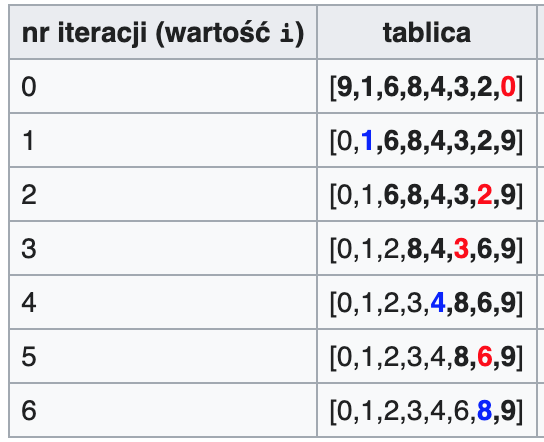
\includegraphics[width=1\textwidth]{selection}
			\caption{{\tiny Sortowanie przez wybieranie. Legenda: czerwony -- minumum, czarny pogrubiony -- elementy do posortowania, niebieski -- elementy na właściwym miejscu.}}
		\end{figure}
	\end{minipage}
\end{frame}

\begin{frame}
	\frametitle{Sortowanie bąbelkowe}
	\begin{block}{Algorytm}
		\begin{enumerate}
		\item Zaczynając od początku listy porównuje się wartości dwóch kolejnych elementów listy. \\
		\item Jeżeli ich kolejność jest prawidłowa, to inkrementuje się indeks o 1.\\
		\item  Jeżeli ich kolejność jest nieprawidłowa, to zamienia się elementy miejscami i inkrementuje się indeks o 1.\\
		\item Gdy dojdzie się do końca listy, to kroki powtarza się od początku do momentu aż cała lista będzie posortowana.
		\end{enumerate}
	\end{block}
	\begin{itemize}
		\item listę przechodzi się tyle razy aż wszystkie elementy będą na swoich miejscach
		\item algorytm ten jest zbyt wolny i niepraktyczny w użyciu
	\end{itemize}
\end{frame}

\begin{frame}
	\frametitle{Sortowanie bąbelkowe}
	\begin{minipage}{0.4\textwidth}
		\begin{varblock}[4.9cm]{{\large \textbf{Sortowanie bąbelkowe}}}
			\begin{tabular}{ >{\centering\arraybackslash} m{3.05cm}| >{\centering\arraybackslash} m{1cm} }
				%\textbf{Sortowanie szybkie} & \\
				Złożoność czasowa pesymistyczna & $n^2$ \\
				\hline
				Złożoność czasowa przeciętna & $n^2$ \\
				\hline
				Złożoność czasowa optymistyczna & $n$ \\
				\hline
				Stabilność & $+$ \\
				\hline
				Złożoność pamięciowa & $1$ \\
			\end{tabular}
		\end{varblock}
	\end{minipage}
	\hspace{0.5cm}
	\begin{minipage}{0.45\textwidth}
		\begin{figure}
			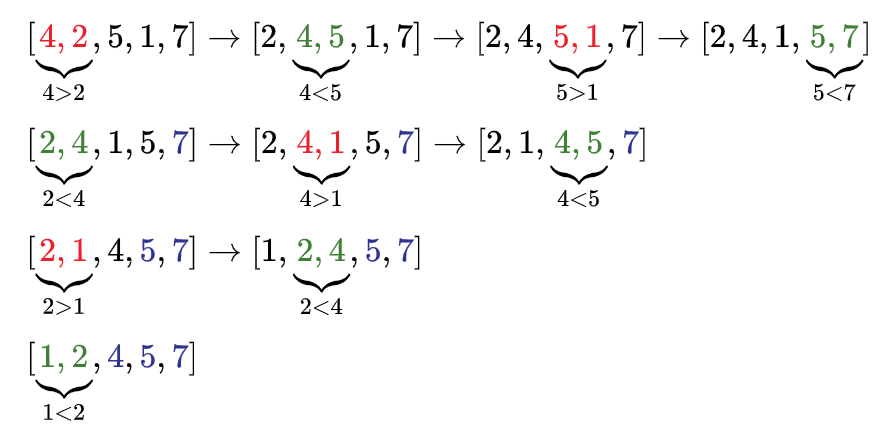
\includegraphics[width=1\textwidth]{bubble}
			\caption{{\tiny Sortowanie bąbelkowe.}}
		\end{figure}
	\end{minipage}
\end{frame}


\begin{frame}
	\frametitle{Sortowanie przez scalanie}
	\begin{block}{Algorytm}
{\footnotesize 		\begin{enumerate}
	 \item Dzieli się początkowy zbiór na kolejne "połowy" dopóki taki podział jest możliwy (tzn. podzbiór zawiera co najmniej dwa elementy).
	 \item Następnie dla każdych dwóch łączonych na danym poziomie podzbiorów definiuje się wskaźniki i porównuje się elementy przez nie wskazywane.
	 \item Elementy łączy się (przenosi na kolejny poziom drzewa) w odpowiedniej kolejności. Przy tym inkrementowany jest wskaźnik tego podzbioru, którego element trafił do podzbioru kolejnego poziomu, po czym wykonuje się następne porównanie na tym samym podzbiorze.
	 \item Porównywanie powtarza się na każdym z poziomów aż do całkowitego posortowania zbioru wyjściowego.
	 \end{enumerate}}
	\end{block}
{\footnotesize 	\begin{itemize}
		\item John von Neumann, 1945
		\item "dziel i rządź"* -- algorytm rekurencyjny
	\end{itemize}}
{\scriptsize *polega na podziale zadania głównego na zadania mniejsze dotąd, aż rozwiązanie stanie się oczywiste\\}
\end{frame}

\begin{frame}
	\frametitle{Sortowanie przez scalanie}
		\begin{minipage}{0.4\textwidth}
	\begin{varblock}[4.9cm]{{\large \textbf{Sortowanie przez scalanie}}}
		\begin{tabular}{ >{\centering\arraybackslash} m{3.05cm}| >{\centering\arraybackslash} m{1cm} }
			%\textbf{Sortowanie szybkie} & \\
			Złożoność czasowa pesymistyczna & $n \cdot logn$ \\
			\hline
			Złożoność czasowa przeciętna & $n \cdot logn$ \\
			\hline
			Złożoność czasowa optymistyczna & $n \cdot logn$ \\
			\hline
			Stabilność & $+$ \\
			\hline
			Złożoność pamięciowa & $n$ \\
		\end{tabular}
	\end{varblock}
\end{minipage}
\hspace{0.5cm}
\begin{minipage}{0.45\textwidth}
		\begin{figure}
		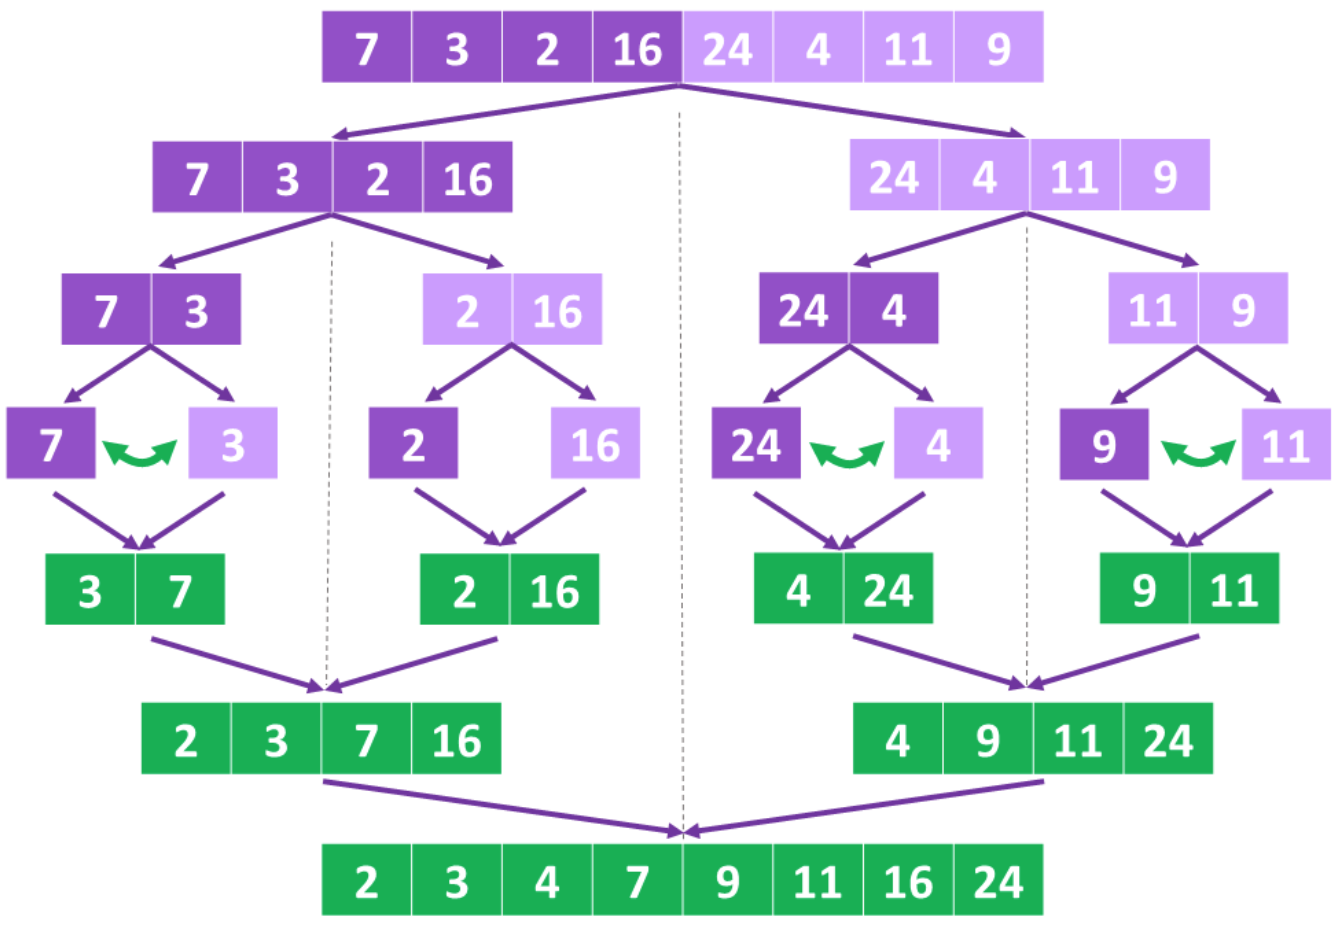
\includegraphics[width=1\textwidth]{merge}
		\caption{{\tiny Sortowanie przez scalanie.}}
		\end{figure}
\end{minipage}
\end{frame}

\begin{frame}
	\frametitle{Sortowanie szybkie}
	\begin{block}{Algorytm}
{\footnotesize 		\begin{enumerate}
%			\item Wybierany jest 1 element -- tzw. piwot.*
%			\item W zależności od wartości piwota dzieli się wyjściową strukturę na podstruktury w ten sposób, że elementy po lewej są mniejsze a po prawej większe od piwota.**
%			\item Pozycjonuje się piwot w odpowiednią pozycję, żeby poprawnie oddzielał te dwie podstruktury.
%			\item Powyższe kroki stosuję się rekursywnie na obu podstrukturach aż do całkowitego posortowania.
\item Określa się pierwszy element listy jako piwot.
\item Definiuje się dwie zmienne pomocnicze -- np. i oraz j -- i ustawia się je odpowiednio na pierwszym i ostatnim elemencie listy.
\item Inkrementuje się i dopóki element lista[i] $>$ piwota.
\item Dekrementuje się j dopóki element lista[j] $<$ piwota.
\item Gdy i $<$ j wtedy zamienia się miejscami elementy lista[i] i lista[j].
\item Powtarza się kroki 3, 4, 5 dopóki i $>$ j.
\item Zamienia się miejscami piwot z elementem lista[j].
\item Kontunuuje się na prawej i lewej podstrukturze aż wszystkie lementy będą na swoich miejscach docelowych.
		\end{enumerate}}
	\bigskip
{\scriptsize 	*wartości równe piwotowi idą na arbitralnie ustalaną stronę \\}
	\end{block}
\end{frame}

\begin{frame}
	\frametitle{Sortowanie szybkie}
		\begin{minipage}{0.4\textwidth}
			\begin{varblock}[4.9cm]{{\large \textbf{Sortowanie szybkie}}}
				\begin{tabular}{ >{\centering\arraybackslash} m{3.05cm}| >{\centering\arraybackslash} m{1cm} }
				%\textbf{Sortowanie szybkie} & \\
				Złożoność czasowa pesymistyczna & $n^2$ \\
				\hline
				Złożoność czasowa przeciętna & $n \cdot logn$ \\
				\hline
				Złożoność czasowa optymistyczna & $n \cdot logn$ \\
				\hline
				Stabilność & $-$ \\
				\hline
				Złożoność pamięciowa & $1$ \\
				\end{tabular}
			\end{varblock}
		\end{minipage}
		\hspace{0.5cm}
		\begin{minipage}{0.45\textwidth}
	\begin{itemize}
	\item wydajny algorytm sortowania -- dobrze zaimplemetowany może być nawet 2-3x szybszy od sortowania przez scalanie czy sortowania z użyciem sterty
	\item najczęściej stosowany algorytm sortowania
	\item link do animacji: \underline{\href{http://algorytmy.ency.pl/tutorial/quicksort}{click}}
\end{itemize}


		\end{minipage}
\end{frame}


\begin{frame}
	\frametitle{Sortowanie przez wstawianie}
	\begin{block}{Algorytm}
			\begin{enumerate}
			\item Począwszy od drugiego elementu (wskaźnik na drugiej pozycji), wybieramy dany element i porównujemy go z każdym elementem z lewej strony (we wstępnie posortowanej części).
			\item Przesuwamy i wstawiamy go na odpowiednie miejsce.
			\item Powtarzamy działanie dla kolejnych elementów ciągu (wskaźnik zawsze przesuwa się o 1 dalej) aż wszystkie elementy będą na swoim miejscu.
		\end{enumerate}
	\end{block}
	\begin{itemize}
		\item algorytm wydajny do sortowania małych struktur
		\item jest bardziej wydajny niż pozostałe algorytmy posiadające złożoność kwadratową
	\end{itemize}
\end{frame}

\begin{frame}
	\frametitle{Sortowanie przez wstawianie}
	\begin{minipage}{0.4\textwidth}
		\begin{varblock}[4.9cm]{{\large \textbf{Sortowanie przez wstawianie}}}
			\begin{tabular}{ >{\centering\arraybackslash} m{3.05cm}| >{\centering\arraybackslash} m{1cm} }
				%\textbf{Sortowanie szybkie} & \\
				Złożoność czasowa pesymistyczna & $n^2$ \\
				\hline
				Złożoność czasowa przeciętna & $n^2$ \\
				\hline
				Złożoność czasowa optymistyczna & $n$ \\
				\hline
				Stabilność & $+$ \\
				\hline
				Złożoność pamięciowa & $1$ \\
			\end{tabular}
		\end{varblock}
	\end{minipage}
	\hspace{0.5cm}
	\begin{minipage}{0.45\textwidth}
				\begin{figure}
					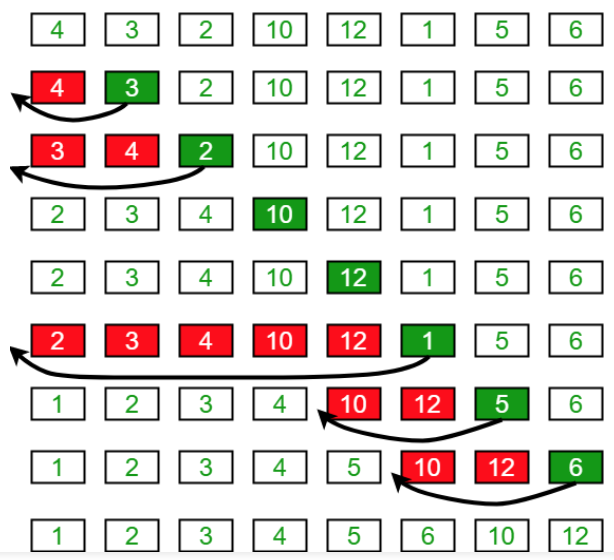
\includegraphics[width=1\textwidth]{insertion}
					\caption{{\tiny Sortowanie przez wstawianie.}}
				\end{figure}
	\end{minipage}
\end{frame}

\begin{frame}
	\frametitle{Sortowanie zliczeniowe}
	\begin{block}{Algorytm}
		
	
{\footnotesize 	\begin{enumerate}
		\item Dla każdej wartości w zbiorze przygotowujemy licznik.
		\item Przeglądamy kolejne elementy zbioru i zliczamy ich wystąpienia w odpowiednich licznikach.
		\item Poczynając od drugiego licznika sumujemy zawartość licznika oraz jego poprzednika*.
		\item Przeglądamy jeszcze raz zbiór wejściowy idąc od ostatniego elementu do pierwszego. Każdy element umieszczamy w zbiorze wynikowym na pozycji równej zawartości licznika dla tego elementu. Po wykonaniu tej operacji licznik zmniejszamy o 1. Dzięki temu następna taka wartość trafi na wcześniejszą pozycję.
	\end{enumerate}}
{\scriptsize * w każdym liczniku otrzymaliśmy ilość wartości mniejszych lub równych numerowi licznika.}
\end{block}
\end{frame}

\begin{frame}
	\frametitle{Sortowanie zliczeniowe}
	\begin{minipage}{0.4\textwidth}
		\begin{varblock}[4.9cm]{{\large \textbf{Sortowanie zliczeniowe}}}
			\begin{tabular}{ >{\centering\arraybackslash} m{3.05cm}| >{\centering\arraybackslash} m{1cm} }
				%\textbf{Sortowanie szybkie} & \\
				Złożoność czasowa pesymistyczna & $n + k$ \\
				\hline
				Złożoność czasowa przeciętna & $n + k$ \\
				\hline
				Złożoność czasowa optymistyczna & $n + k$ \\
				\hline
				Stabilność & $+$ \\
				\hline
				Złożoność pamięciowa & $n + k$ \\
			\end{tabular}
		\end{varblock}
	\end{minipage}
	\hspace{0.5cm}
	\begin{minipage}{0.45\textwidth}
			\begin{figure}
			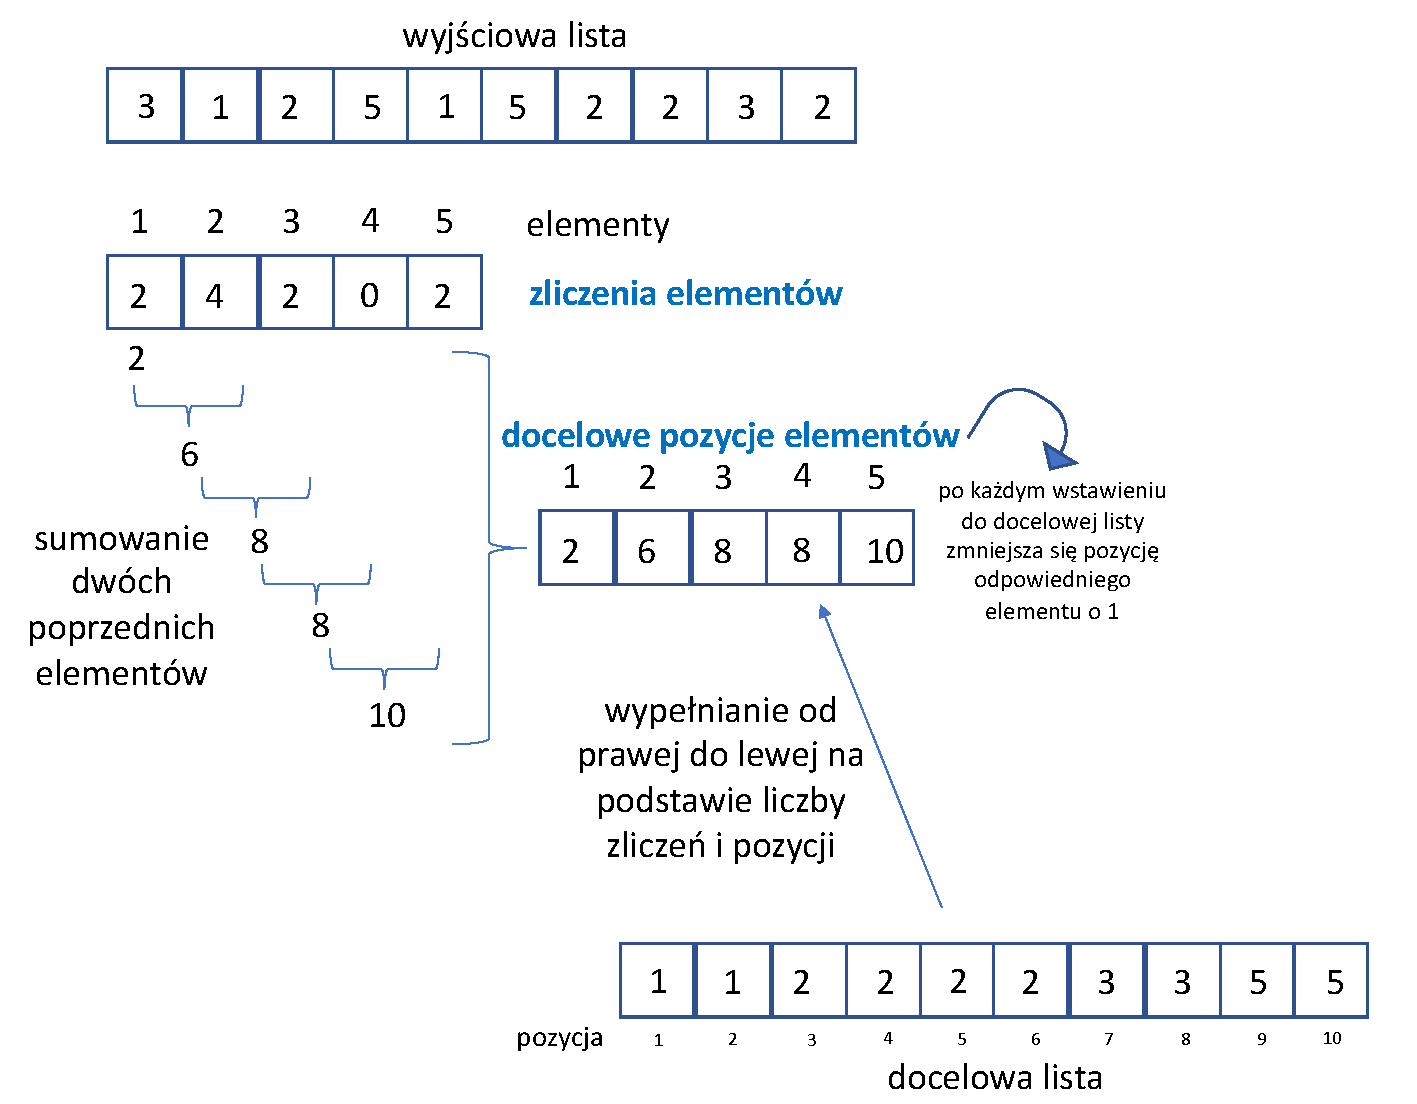
\includegraphics[width=1.2\textwidth]{counting}
			\caption{{\tiny Sortowanie zliczeniowe.}}
		\end{figure}
	\end{minipage}
\end{frame}

\begin{frame}
	\frametitle{Porównanie wybranych algorytmów sortowania}
	\begin{table}
		\caption{Porównanie parametrów wybranych algorytmów.}
		\begin{tabular}{c c c c c c}
			\toprule
			\textbf{Rodzaj} & \textbf{Złoż.} & \textbf{Złoż.} & \textbf{Złoż.} & \textbf{Stabilność} & \textbf{Złoż.}\\
			\textbf{sort.} & \textbf{czas.} & \textbf{czas.} & \textbf{czas.} & \textbf{} & \textbf{pamięc.}\\
			\textbf{} & \textbf{pes.} & \textbf{przec.} & \textbf{opt.} & \textbf{} & \textbf{}\\
			\midrule
			p. wybieranie & $n^2$ & $n^2$  & $n$ & $-$ & $1$ \\
			bąbelkowe & $n^2$ & $n^2$  & $n$ & $+$ & $1$\\
			p. scalanie & $n \cdot logn$ & $n \cdot logn$  & $n \cdot log n$& $+$ & $n$ \\
			szybkie & $n^2$ & $n \cdot logn$  & $n \cdot logn$ & $-$ & $1$ \\
			p. wstawianie & $n^2$ & $n^2$  & $n$ & $+$ & $1$ \\
			zliczeniowe & $n + k$ & $n + k$  & $n + k$ & $+$ & $n + k$ \\
			\bottomrule
		\end{tabular}
	\end{table}
	{\tiny n -- liczba elementów struktury danych, k -- liczba możliwych wartości\\ 
		Użyta notacja to O() -- służy do oznaczania rzędu wielkości (górnego ograniczenia tempa wzrostu) funkcji}
\end{frame}


\begin{frame}
	\frametitle{Zastosowania wyszukiwania i sortowania}
	Algorytmy wyszukiwania i sortowania są stosowane w celu:
	\begin{itemize}
		\item uporządkowania danych
		\item zwiększenia wydajności aplikacji (szybsze wykonywanie operacji, wydajniejsze działanie programów)
		\item prezentacji danych w sposób czytelniejszy dla człowieka
	\end{itemize}
\bigskip
\bigskip
{\scriptsize Wykorzystują je interaktywne aplikacje, np. webowe, desktopowe, do księgowości, naukowe, zakupowe, platformy streamingowe, portale i wiele innych.\\
Posiadają one wbudowane moduły wyszukiwania i sortowania żeby ułatwić użytkownikowi znalezienie porządanego (optymalnego) rozwiązania. \\}
\end{frame}




%-------------------------------  SEKCJA O BIBLIOTECE STREAM JAVA   -----------------



\section{Pytanie nr 34} % Sections can be created in order to organize your presentation into discrete blocks, all sections and subsections are automatically printed in the table of contents as an overview of the talk
%------------------------------------------------

\subsection{Przetwarzanie strumieniowe (środki pakietu java.util.stream).} % A subsection can be created just before a set of slides with a common theme to further break down your presentation into chunks

\begin{frame}
	\frametitle{Pakiet java.util.stream}
	\begin{center}
		{\Huge Pakiet java.util.stream}
	\end{center}
\end{frame}


\begin{frame}
\frametitle{Pakiet java.util.stream}

\end{frame}

%------------------------------------------------
%
%\begin{frame}
%\frametitle{Bullet Points}
%\begin{itemize}
%\item Lorem ipsum dolor sit amet, consectetur adipiscing elit
%\item Aliquam blandit faucibus nisi, sit amet dapibus enim tempus eu
%\item Nulla commodo, erat quis gravida posuere, elit lacus lobortis est, quis porttitor odio mauris at libero
%\item Nam cursus est eget velit posuere pellentesque
%\item Vestibulum faucibus velit a augue condimentum quis convallis nulla gravida
%\end{itemize}
%\end{frame}
%
%%------------------------------------------------
%
%\begin{frame}
%\frametitle{Blocks of Highlighted Text}
%\begin{block}{Block 1}
%Lorem ipsum dolor sit amet, consectetur adipiscing elit. Integer lectus nisl, ultricies in feugiat rutrum, porttitor sit amet augue. Aliquam ut tortor mauris. Sed volutpat ante purus, quis accumsan dolor.
%\end{block}
%
%\begin{block}{Block 2}
%Pellentesque sed tellus purus. Class aptent taciti sociosqu ad litora torquent per conubia nostra, per inceptos himenaeos. Vestibulum quis magna at risus dictum tempor eu vitae velit.
%\end{block}
%
%\begin{block}{Block 3}
%Suspendisse tincidunt sagittis gravida. Curabitur condimentum, enim sed venenatis rutrum, ipsum neque consectetur orci, sed blandit justo nisi ac lacus.
%\end{block}
%\end{frame}
%
%%------------------------------------------------
%
%\begin{frame}
%\frametitle{Multiple Columns}
%\begin{columns}[c] % The "c" option specifies centered vertical alignment while the "t" option is used for top vertical alignment
%
%\column{.45\textwidth} % Left column and width
%\textbf{Heading}
%\begin{enumerate}
%\item Statement
%\item Explanation
%\item Example
%\end{enumerate}
%
%\column{.5\textwidth} % Right column and width
%Lorem ipsum dolor sit amet, consectetur adipiscing elit. Integer lectus nisl, ultricies in feugiat rutrum, porttitor sit amet augue. Aliquam ut tortor mauris. Sed volutpat ante purus, quis accumsan dolor.
%
%\end{columns}
%\end{frame}
%
%%------------------------------------------------
%%\section{Second Section}
%%------------------------------------------------
%
%\begin{frame}
%\frametitle{Table}
%\begin{table}
%\begin{tabular}{l l l}
%\toprule
%\textbf{Treatments} & \textbf{Response 1} & \textbf{Response 2}\\
%\midrule
%Treatment 1 & 0.0003262 & 0.562 \\
%Treatment 2 & 0.0015681 & 0.910 \\
%Treatment 3 & 0.0009271 & 0.296 \\
%\bottomrule
%\end{tabular}
%\caption{Table caption}
%\end{table}
%\end{frame}
%
%%------------------------------------------------
%
%\begin{frame}
%\frametitle{Theorem}
%\begin{theorem}[Mass--energy equivalence]
%$E = mc^2$
%\end{theorem}
%\end{frame}
%
%%------------------------------------------------
%
%\begin{frame}[fragile] % Need to use the fragile option when verbatim is used in the slide
%\frametitle{Verbatim}
%\begin{example}[Theorem Slide Code]
%\begin{verbatim}
%\begin{frame}
%\frametitle{Theorem}
%\begin{theorem}[Mass--energy equivalence]
%$E = mc^2$
%\end{theorem}
%\end{frame}\end{verbatim}
%\end{example}
%\end{frame}
%
%%------------------------------------------------
%
%\begin{frame}
%\frametitle{Figure}
%Uncomment the code on this slide to include your own image from the same directory as the template .TeX file.
%%\begin{figure}
%%\includegraphics[width=0.8\linewidth]{test}
%%\end{figure}
%\end{frame}
%
%%------------------------------------------------
%
%\begin{frame}[fragile] % Need to use the fragile option when verbatim is used in the slide
%\frametitle{Citation}
%An example of the \verb|\cite| command to cite within the presentation:\\~
%
%This statement requires citation \cite{p1}.
%\end{frame}
%
%%------------------------------------------------
%
%\begin{frame}
%\frametitle{References}
%\footnotesize{
%\begin{thebibliography}{99} % Beamer does not support BibTeX so references must be inserted manually as below
%\bibitem[Smith, 2012]{p1} John Smith (2012)
%\newblock Title of the publication
%\newblock \emph{Journal Name} 12(3), 45 -- 678.
%\end{thebibliography}
%}
%\end{frame}
%
%%------------------------------------------------
%
%\begin{frame}
%\Huge{\centerline{The End}}
%\end{frame}

%----------------------------------------------------------------------------------------

\end{document} 